\section{Knowledge Graph Development Process}

The second chapter of this document aims to describe, in a detailed way, the KG development process. The sections below describe each phase of the KG building project, reporting for each phase, the description of the datasets and their evolution respect the previous phases, the schema construction which will generate the KG ontology in the end, as well as the description of the procedures adopted to manage the data and finally achieve those results. Moreover for each phase is reported an evaluation section, which aims to evaluate the quality of the results achieved at the end of each phase. 

\subsection{Scope Definition}

As the main place of living and the main carrier of "living", which is one of the four major human behaviors of clothing, food, housing and transportation, houses provide people with the material basis of basic living while carrying rich cultural connotations such as architectural culture, living etiquette culture and family culture. As one of the basic needs of human beings, the purchase of a house has become a common issue in our society today. The demand for education has led to the hot demand for school district houses; the superstition of feng shui makes people think twice about the house type before buying a house; besides, the demand for traffic around the house also varies from person to person; the different economic conditions also make the expected area of the house vary greatly; the expectation of future life and other personalized needs for buying a house have also become important factors to be considered.


Based on this, the project aims to provide a unified, comprehensive and structured query solution for the query by cleaning, organizing and fusing the official and authoritative data from the Internet based on the knowledge graph method through the inputted needs related to home purchase (e.g. price range, personality needs, house type consideration). The solution can effectively provide an effective and reasonable query structure for home purchase needs that meet the requirements of the paradigm, which helps reduce the customer's decision space and provides a key theoretical foundation and technical support for improving people's living standards and happiness.


Our data is sampled from the 58 Tongcheng classified information service integration platform, which can provide home buyers with authoritative, reliable, complete and comprehensive information on the basis of home buying. We narrow down the data set by calling the search interface of the website to query specific data, use python scripts to sample the website data and clean it to make it structured; we construct our heterogeneous database group by sampling and cleaning under different search restrictions and reasonably discarding the features of the result data, which is the data source of the project.




Our project is to be implemented according to the following steps:
~\\
\item
 \textbf{Informal Modeling}. This section is dedicated to the Informal Modeling phase description.  The Section is divided in Schema and Data level in order to report the details of the elements involved in the generation of the schema, as well as the description of the datasets evolution in this phase.  Moreover a specif section, one for each level, reports the difference between the elements defined in this phase and the definitions in the previous phase, analyzing in this way the variance in the different phase.
 ~\\
 \item
 \textbf{Formal Modeling}. This section is dedicated to the Formal Modeling phase description.  The Section is divided in Schema and Data level in order to report the details regarding both the ontology generated and the datasets version in the current phase.
 ~\\
 \item  
 \textbf{Data integration}. This section is dedicated to the Data Integration phase.
\subsection{Inception}
This section is dedicated to the Inception phase description. Here are reported the initial definitions for CQs (Competency Queries), initial datasets collected and the relative metadata. For each of those elements the procedures
and the tools adopted to achieve the results, have to be reported in the sections below.

\subsubsection{Scenarios of usages}

\item
\textbf{Actor}: Jerry, 20
\item
\textbf{Scenario}: Jerry is an undergraduate from Jilin University who is about to graduate. After graduation, he plans to continue to study and work in Changchun and settle down. He is full of enthusiasm for life. In addition to studying and working, he likes to stroll around vibrant places. In the hard work phase of entering society, he will not consider starting a family for the time being, so he only wants to buy a single apartment.


\item
\textbf{Actor}: Tom & Mary
\item
\textbf{Scenario}: Tom, 30, has worked in Changchun for many years and has a stable and expensive income. Mary, 28, is a full-time housewife. Recently, their family had a happy event ——birth of a twin. But now their house areas only 60 square meters, which is not enough for the basic living needs of a family of four. They want to buy a three-bedroom and one-living school district house of more than 120 square meters in downtown Changchun.


\item
\textbf{Actor}: Alex, 60
\item
\textbf{Scenario}: As a successful person who has worked hard for decades in the business world, Alex has reached the age of retirement. He is tired of the hustle and bustle of the city centre and wants to find the joy of life with his wife. They hope to buy a villa or townhouse in the suburbs of Changchun to get closer to nature.

\subsubsection{CQs definition}
This subsection is dedicated to the definition of the Competency Queries. They have to be listed and explained with details in order to have the information they bring, as clear as possible. This section plays a crucial role in the project description due to the fact that the CQs are the starting point to define the single objects/entities involved in the KG. For this reason the CQs will be used in the next phases as evaluation base to define the quality of the outcomes of each phase. 


\newcommand{\tabincell}[2]{\begin{tabular}{@{}#1@{}}#2\end{tabular}}
\begin{table}
    \Large
    \caption{Query Description}  
    \begin{center}
    \begin{tabular}{|p{2.3cm}|p{12.1cm}|}    %{|l|l|}
    %%\resizebox{\textwidth}{12mm}
    %%表格的宽度需要调整
    \hline  
    Actor & Query \\  
    \hline  
    Jerry & \tabincell{l}{As a newly graduated undergraduate, his financial\\ strength is still weak, and he has reasonable \\expectations about the average price of a house when \\purchasing a house.} \\
    \hline
    Jerry & \tabincell{l}{Expecting to purchase a single apartment since there is\\ no need to start a family.} \\
    \hline
    Jerry & \tabincell{l}{Due to his personal hobby of going to lively places for\\ shopping, he has certain requirements for the traffic\\ around the house.}\\
    \hline
    Tom Mary & \tabincell{l}{With years of stable work experience, they have a good\\ financial base and can consider buying a high quality\\ house with a high price.} \\
    \hline
    Tom Mary & \tabincell{l}{With the new addition to the family, the existing house\\ is too small to meet the needs of a family of four, so \\when buying a house, they consider the need for a\\ larger area.} \\
    \hline
    Tom Mary & \tabincell{l}{When the baby grows up, the parents need to have\\ independent space, and the parents need to allocate a \\suite to each of the two children on the basis of a \\separate room, so they need to purchase a house with\\ three rooms and a hall.} \\
    \hline
    Tom Mary & \tabincell{l}{The two couples showed a desire to purchase a house in\\ the city center.}\\
    \hline
    Alex & \tabincell{l}{Tired of the city center and wanting to live quietly with\\ his wife, he has the desire to live away from the hustle\\ and bustle of the city center and be close to nature, \\and is considering purchasing a house in a location far \\from the city.} \\
    \hline
    Alex & \tabincell{l}{As successful businessmen, they are naturally \\well-off, and villas and townhouses are the types of\\ houses they want to buy.} \\
    \hline  
    \end{tabular}
    \end{center}
    \end{table} 
    
    
\subsubsection{Initial Datasets description}
Since we concentrate on offering suitable houses for buyers in Changchun,we decided to use the data of houses located in Changchun. In order to get enough data about houses, we browsed several webs and finally chose the website \url{https://cc.58.com/xinfang/} which is one of the biggest websites to buy houses. We utilized BeautifulSoup to crawl data from it. And the listed houses contain information about its name,its location,its type,its area and its price per square meter. In order to combine the transportation information with information of house, We used the same way to crawl the dataset of transportation in the website \url{https://cc.fang.ke.com/loupan}, which contains the opening time and average price of houses as well.
\subsubsection{Datasets metadata documentation}
We have collected three datasets and are overall information of the houses,additional information of the houses and light railways and their relative houses.  here are the matadata tables about them respectively.
    \begin{table}[!htbp]  
    \Large
    \caption{Overall information of the houses}  
    \begin{center}
    \begin{tabular}{|p{4.3cm}|p{13cm}|}%{|l|l|}  
    \hline  
    Field Name & Description \\  
    \hline  
    Dataset Description & This dataset concludes overall information of the houses \\
    \hline
    Dataset Source & 58.com \\  
    \hline
    Language & Chinese \\
    \hline
    Ownership & 58.com \\
    \hline
    URL & \url{https://cc.58.com/xinfang/} \\
    \hline
    Format & Json \\
    \hline  
    Attributes & name,location,type,area and price \\
    \hline
    \end{tabular}
    \end{center}
    \end{table}  
    
    \begin{table}[!htbp]  
    \Large
    \caption{additional information of the houses}  
    \begin{center}
    \begin{tabular}{|p{4.3cm}|p{13cm}|}%{|l|l|}  
    \hline  
    Field Name & Description \\  
    \hline  
    Dataset Description & This dataset concludes additional information of the houses \\
    \hline
    Dataset Source & ke.com \\  
    \hline
    Language & Chinese \\
    \hline
    Ownership & ke.com \\
    \hline
    URL & \url{https://cc.fang.ke.com/loupan} \\
    \hline
    Format & Json \\
    \hline 
    Attributes & name,price and the opening time \\
    \hline
    \end{tabular}
    \end{center}
    \end{table}  
    
    \begin{table}[!htbp]  
    \Large
    \caption{light railways and their relative houses}  
    \begin{center}
    \begin{tabular}{|p{4.3cm}|p{13cm}|}%{|l|l|}  
    \hline  
    Field Name & Description \\  
    \hline  
    Dataset Description & This dataset concludes some local light railways and houses on sale nearby.  \\
    \hline
    Dataset Source & ke.com \\  
    \hline
    Language & Chinese \\
    \hline
    Ownership & ke.com \\
    \hline
    URL & \url{https://cc.fang.ke.com/loupan/li8740130349630421/#8740130349630421}(an example of the concrete format ) \\
    \hline
    Format & Json \\
    \hline  
    Attributes & name,price and the opening time \\
    \hline
    \end{tabular}
    \end{center}
    \end{table}  

    \begin{table}[!htbp]  
    \Large
    \caption{The information of schools}  
    \begin{center}
    \begin{tabular}{|p{4.3cm}|p{13cm}|}%{|l|l|}  
    \hline  
    Field Name & Description \\  
    \hline  
    Dataset Description & This dataset concludes the information of schools in Changchun.  \\
    \hline
    Dataset Source & Amap \\  
    \hline
    Language & Chinese \\
    \hline
    Ownership & Amap \\
    \hline
    URL & \url{https:https://restapi.amap.com/v3/place/text?}(and with some addtional parameters) \\
    \hline
    Format & Json \\
    \hline  
    Attributes & name,type,longitude,latitude,address \\
    \hline
    \end{tabular}
    \end{center}
    \end{table}  
    
    
\subsubsection{Datasets collection process}
There is no available database to construct a knowledge graph about buying houses in Changchun, so we tried to use web-scraping tools to get the data from the website mentioned in 2.2.2. Considering the convenience of Python in web-scraping, we used the 'BeautifulSoup' package of Python to obtain the acquired data. And in the Python script we extract the important attributes about each house as mentioned above. And to identify whether a house is school district house or not we used the API of Amap to obtain all the information of schools in Changchun. Finally, we got all our initiative datasets.

%\subsubsection{Inception level evaluation}
%The last section of the Inception phase report the evaluation %of the outcomes obtained in this phase, through specif %evaluation metrics. 
\subsection{Informal Modeling}
This section is dedicated to the Informal Modeling phase description. The Section is divided in Schema and Data level in order to report the details of the elements involved in the generation of the schema, as well as the description of the datasets evolution in this phase. Moreover a specif section, one for each level, reports the difference between the elements defined in this phase and the definitions in the previous phase, analyzing in this way the variance in the different phases. 

\subsubsection{Schema level}
The schema level in this phase report the first informal definition of the ETypes and of the EER model constructed using them. 

\paragraph{ETypes and EER Model definition}\mbox{}\\
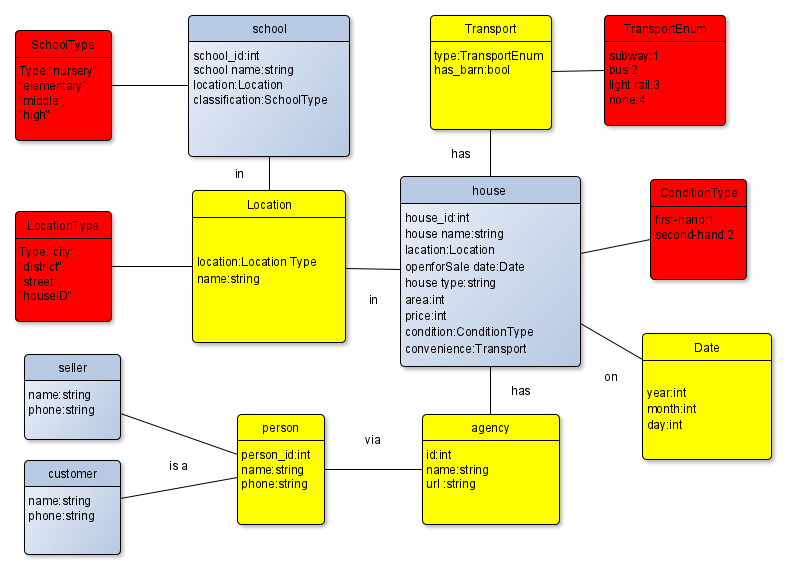
\includegraphics[width=18cm]{student codebook/sections/EER2.png}
    \caption{EER model for buy-a-house project}

To fulfill the requirement of buying a house, we built the EER model diagram above.
Among them, we use houses, sellers, buyers and schools as the core entities, because we will focus on completing the process of buying houses and dealing with the housing demand of the school district.As the most basic information of the event, the housing information should be as comprehensive as possible, so we collected the information including name, location, open-for-sale time, area, house type, price, convenience and so on.In addition, we collected the data of schools in Changchun, including school name, location and school type.We also enumerated which agent to provide the corresponding house information.

\paragraph{Variance respect CQs definition}\mbox{}\\
During the Inception phase, we discussed and developed a series of house-buying scenarios that resulted in several CQ definitions.However, after building the EER map to account for the actual situation and considering the possibility of data acquisition, our EER model may not satisfy some queries very well.For example,the definition of suburban and urban areas from metadata is not clear enough,which make it difficult to query suburban and urban homes.

\subsubsection{Data level}
The data level section in this phase reports the evolution of the datasets collected previously, reporting the metadata information for each new data, or new version of data, obtained.

\paragraph{Datasets management process}\mbox{}\\
In the formal process we got the price information about the houses and stored it in the first dataset. However, the price information in the first dataset have different kinds of forms. Some are the avarage price of the house and some are the lowest price of the house. So it's hard to get a uniform format of the result when querying the result. In this case we used the price information of the 3rd dataset which is all about the average price and replaced the origin one. And since the information of price is stored in the first dataset. We delete that in the 3rd one.And due to the format of the website we used, it's possible to get data without the property of house type and got a wrong data instead. And we found it's because they were office building so we delete the original wrong content and changed its type to office building.

\paragraph{Datasets metadata documentation}\mbox{}\\
Since in the process of cleaning datasets we only changed several value of their attributes, the datasets metadata is same as the one we given in the 2.2.4. And the concrete changes in attributes we have listed in the previous part 2.3.2.1.
\paragraph{Variance respect Inception datasets}\mbox{}\\
Since the features in the dataset are almost all literal quantities, it is difficult to use a quantitative criterion to measure the variance, so the variance-related issues are not elaborated much in this section.

\subsubsection{Informal Modeling Evaluation}
This project measures the reliability of the informal model in terms of the accuracy of the query results, i.e., the query results should not conflict with the features in the dataset. Since query requirements are diverse and the query results may exceed human common sense, reliability should be used as the evaluation index of the informal model, and too many subjective factors should not be added.
\subsection{Formal Modeling}
This section is dedicated to the Formal Modeling phase description. The Section is divided in Schema and Data level in order to report the details regarding both the ontology generated and the datasets version in the current phase.

\subsubsection{Schema level}
The schema level section in the current phase, reports the detailed description of the ontology generation.

\paragraph{Ontology definition}\mbox{}\\
The first step in the process of developing an ontology schema is to search for other reference ontologies. In this project, there are few reference examples, but we have the a priori knowledge that the data crawled from different websites are cell names and their related attributes. It is common knowledge that, within a given range, cell names can help people to identify different cells, so cell names and cell entities correspond to each other. In addition, the cell names are given by the cell entities themselves, and the websites are only responsible for collecting and organizing the relevant information without subjective processing, so the cell name attribute fields of the heterogeneous databases completely overlap and there is no ambiguity, which brings convenience to the data level fusion.


A simplest approach is adopted in this project, i.e., multiple databases are stitched together as the database after fusion based on the cell name restriction. The pseudo python code of the algorithm is shown 
as follows.


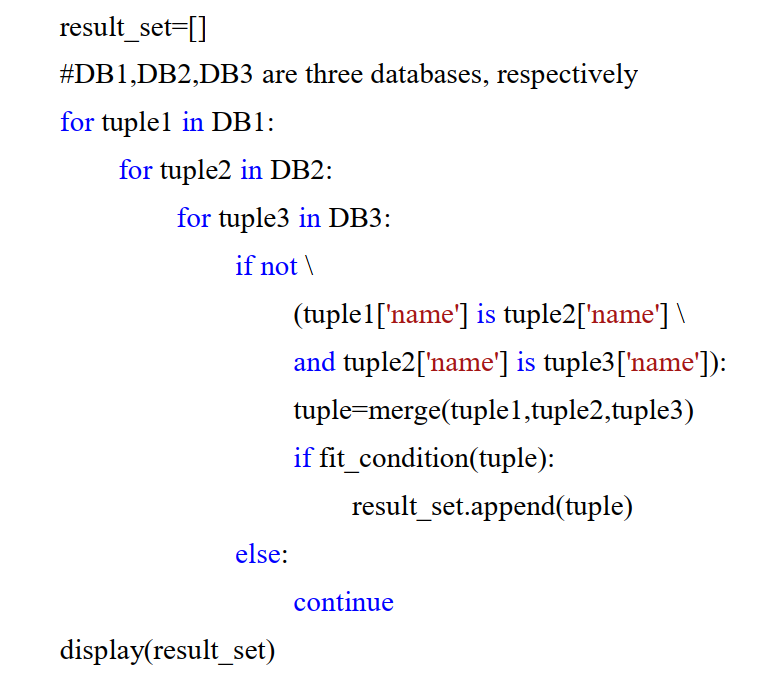
\includegraphics[width=8cm]{student codebook/sections/figure.png}
    \caption{python pseudo-code of our algorithm}




\subsection{Data integration}
This section is dedicated to the Data Integration phase description.

\subsubsection{Data integration operations and tool}
Matching and splicing based on the same domain attributes of heterogeneous databases and filtering based on query conditions are the main strategies for fusion in this project. The cell name attribute serves as a bridge between different databases, and its uniqueness and identifiability facilitate the implementation of the fusion strategy. In addition, filtering based on personalized query statements supports the export of correct results.

\subsubsection{Variance respect Formal Modeling datasets}
The last section of the data integration phase aims to describe the variance, analyzing the differences, between the datasets integrated with the ontology, in the data integration platform which contain the KG, and the datasets collected in the previous phase. This analysis can highlight the results of the operations performed during the final phase of the data integration process.
